\documentclass{article}

% if you need to pass options to natbib, use, e.g.:
% \PassOptionsToPackage{numbers, compress}{natbib}
% before loading nips_2017
%
% to avoid loading the natbib package, add option nonatbib:
% \usepackage[nonatbib]{nips_2017}


% to compile a camera-ready version, add the [final] option, e.g.:
\PassOptionsToPackage{numbers, compress}{natbib}
\usepackage[final]{nips_2017}



\usepackage[utf8]{inputenc} % allow utf-8 input
\usepackage[T1]{fontenc}    % use 8-bit T1 fonts
\usepackage{hyperref}       % hyperlinks
\usepackage{url}            % simple URL typesetting
\usepackage{booktabs}       % professional-quality tables
\usepackage{amsfonts}       % blackboard math symbols
\usepackage{nicefrac}       % compact symbols for 1/2, etc.
\usepackage{microtype}      % microtypography
\usepackage{amsmath}
\usepackage{algorithm}
\usepackage[noend]{algpseudocode}
\usepackage{subfig}
\usepackage{graphicx}

\newcommand{\mc}{\mathcal}
\newcommand{\mb}{\mathbb}
\newcommand{\rar}{\rightarrow}
\newcommand{\sbf}[1]{{\textbf{#1}}}
\newcommand{\sn}[1]{{\sf{#1}}}
\newcommand{\e}{{\sf e}}
\newcommand{\f}{{\sf f}}
\newcommand{\Pdest}{P_{\text{\sn{dest}}}}
\makeatletter
\def\BState{\State\hskip-\ALG@thistlm}
\makeatother

\title{CSE 546 Project Milestone: \\ {Risk-Sensitive Reinforcement and Inverse Reinforcement Learning}}

\author{
  Tanner Fiez \\
  Department of Electrical Engineering \\
  University of Washington \\
  % Seattle, WA \\
  \texttt{fiezt@uw.edu} \\
}

\begin{document}

\maketitle

\section{Introduction}
Reinforcement learning algorithms have historically modeled agents as expected utility maximizers. This modeling paradigm thus considers agents as rational decision makers. A rational decision maker can be described as \emph{risk-neutral}. However, extensive work in behavior psychology, cognitive science, and economics has shown that humans are inherently irrational decision makers acting according to both a reference point and an internal set of risk preferences. This phenomenon has revealed that humans distort event probabilities and value losses and gains asymmetrically. Specifically, low probability events are overestimated and high probability events are underestimated, and losses are weighed more heavily than gains. Owing to these properties, humans tend to be risk-seeking in losses and risk-averse in gains. See Section \ref{example} for a concrete example.

In \cite{DBLP:journals/corr/ShenTSO13} a reinforcement learning framework to model risk-sensitive decision making was created leveraging behavioral models of human decision making. In \cite{mazumdar:2017aa} and \cite{ratliff:2017aa} a risk-sensitive inverse reinforcement learning framework was developed. This project will focus on the reinforcement learning problem and time permitting explore the inverse reinforcement learning problem. The goal of the project is to apply the methods to the New York Taxi dataset\footnote{The New York Taxi dataset is available at \url{https://publish.illinois.edu/dbwork/open-data/}}. The work leading up to the project milestone has been focused on implementing and testing the risk-sensitive reinforcement learning algorithm in a synthetic grid-world environment, formulating the Markov Decision Process (MDP) for taxi drivers, and preprocessing the taxi data to create the underlying MDP for the environment. The bulk time spent on the project thus far has been devoted to the latter two tasks.


\section{Risk-Sensitive Reinforcement Learning}
Sequential decision making problems can often be formulated as an MDP that can be solved via dynamic programming algorithms such as value iteration, policy iteration, and Q-value iteration. These methods however, require that transition probabilities and event outcomes are known a priori. In practice these quantities are typically unknown and thus a policy must be gradually improved as an agent explores an environment. One of the most popular reinforcement learning algorithms to do this is called Q-learning \cite{sutton1998reinforcement}. The Q-learning algorithm iteratively updates the Q-function, a mapping from state-action pairs to value estimates, by taking steps in the direction of an error-like term called the temporal difference. The novel contribution of \cite{DBLP:journals/corr/ShenTSO13} was to extend this method by applying a transformation to the temporal difference term with a value function obeying certain properties and coming from the class of functions that have been developed to model human behavior, while maintaining convergence guarantees. Through applying the value function to the temporal difference term, a nonlinear transformation is applied not only to the rewards, but also to the transition probabilities. This is significant given that this is precisely what humans have been observed to do when making decisions.


\subsection{Algorithm}
The complete procedure for risk-sensitive Q-learning with a finite horizon and a single episode is in Algorithm \ref{risk}. For a more detailed description see Section \ref{alg_desc}.
\begin{algorithm}
\caption{Risk-Sensitive Q-Learning}\label{risk}
\begin{algorithmic}[1]
\Procedure{RiskSensitiveQLearning}{}
\State $\textit{Initialize} \ Q(s, a) = 0 \ \textit{and} \ N(s, a) = 0 \ \forall s, a.$
\For{$t = 1$ to $T$}
    \State $a_t \sim \pi(a|s_t)$
    \State $N(s_t, a_t) = N(s_t, a_t) + 1$
    \State $\alpha_t(s_t, a_t) = 1/N(s_t, a_t)$
    \State $Q_{t+1}(s_t, a_t) = Q_t(s_t, a_t) + \alpha_t(s_t, a_t)\left[u(r_t + \gamma \max_a Q_t(s_{t+1}, a_t) - Q_t(s_t, a_t))\right]$
    \EndFor
\EndProcedure
\end{algorithmic}
\end{algorithm}
\vspace{-4mm}
\subsection{Simulations}
In order to test the implementation of the risk-sensitive Q-learning algorithm we created a synthetic environment called Grid-World. In this environment each state is given by a tile in the grid and the possible actions are the the compass directions (N, E, S, W). The terminal states were set to be the upper left and lower right corners of the grid. Fig.~\ref{fig:sim} provides an example of the results. We designed the environment, which can be thought of as the underlying MDP, very simply to verify the algorithm was learning correctly. Thus transitions were deterministic, i.e. when an action is chosen the agent goes to the expected next state, and each action incurred reward of $-1$ except in the terminal states the reward was $0$. We then used the prospect value function with all risk-parameters set to $1$ which reduces the problem to standard q-learning. Thus the solution that should be learned is to take the Manhattan path to the nearest terminal state, and we indeed see this is the case. More interesting examples can be designed to show how risk-preferences will change the policy that is learned, but we have verified the algorithm is implemented correctly. Detailed results are provided in Section~\ref{sim}
\begin{figure}[H]
    \centering
    \subfloat[][Q-value function results.]{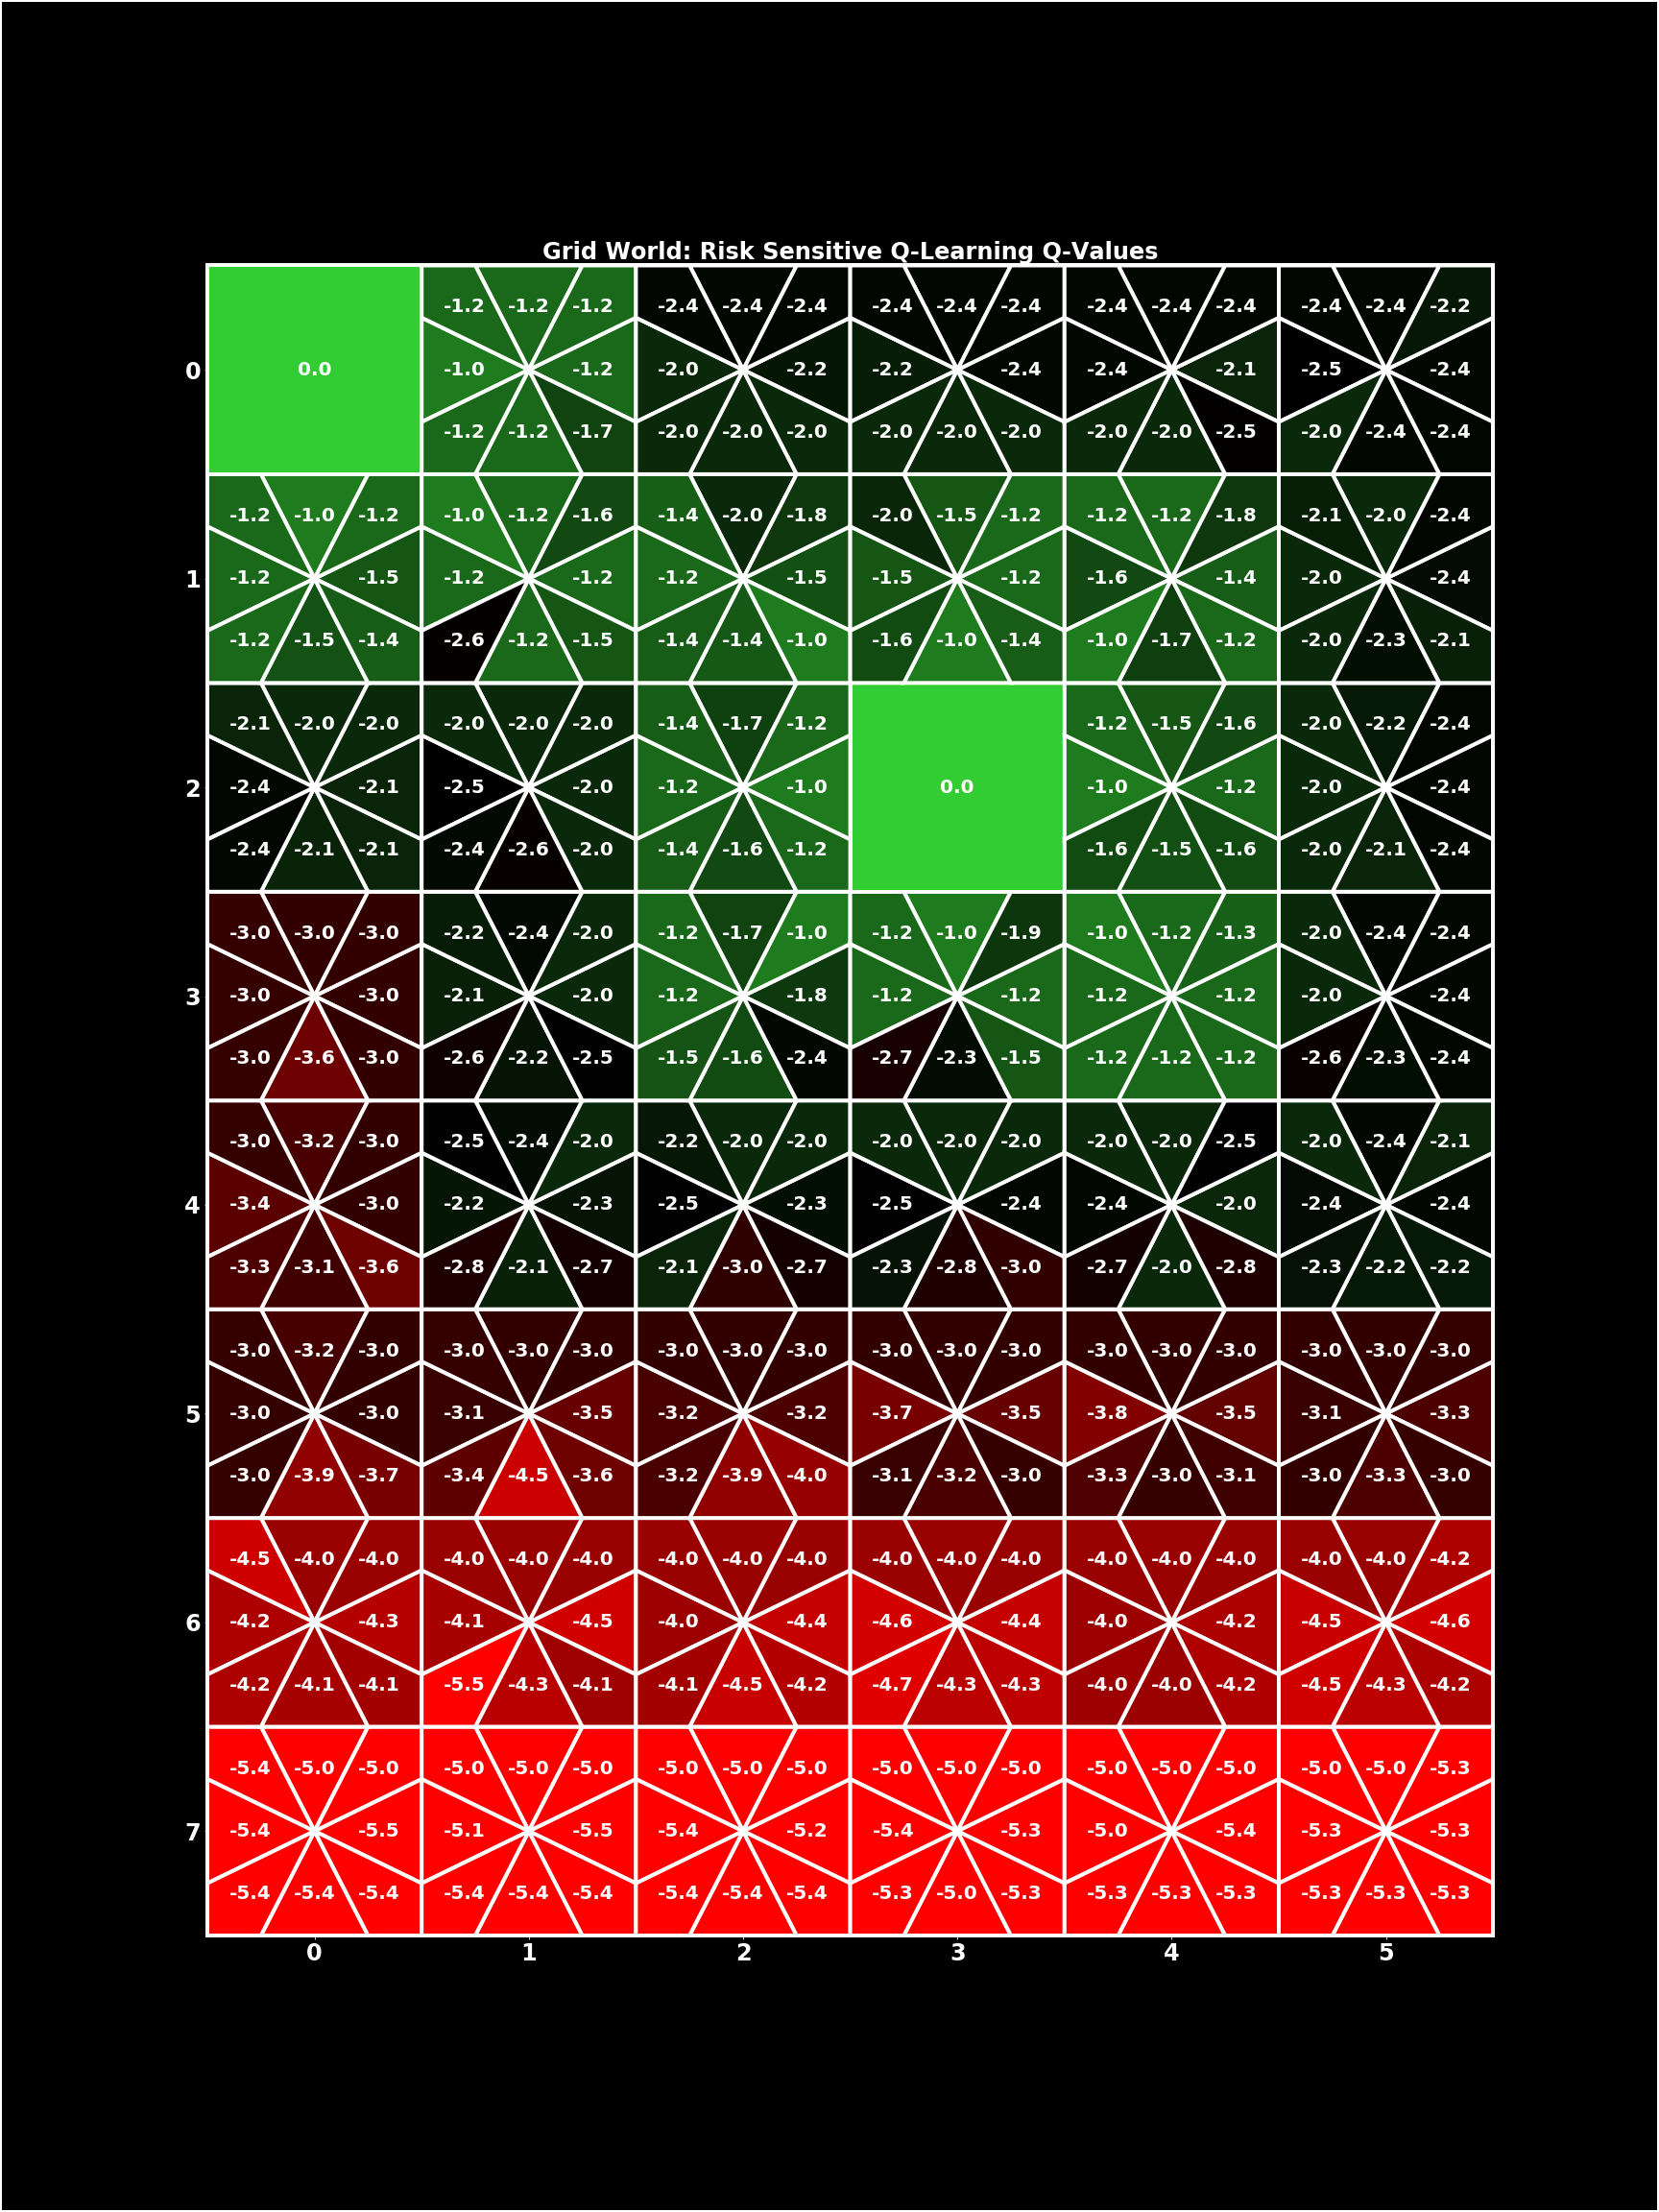
\includegraphics[width=0.5\linewidth]{../figs/Grid_World_Risk_Sensitive_QLearning_QValues}\label{fig:sim1}}\hfill
    \subfloat[][Value function results and policy.]{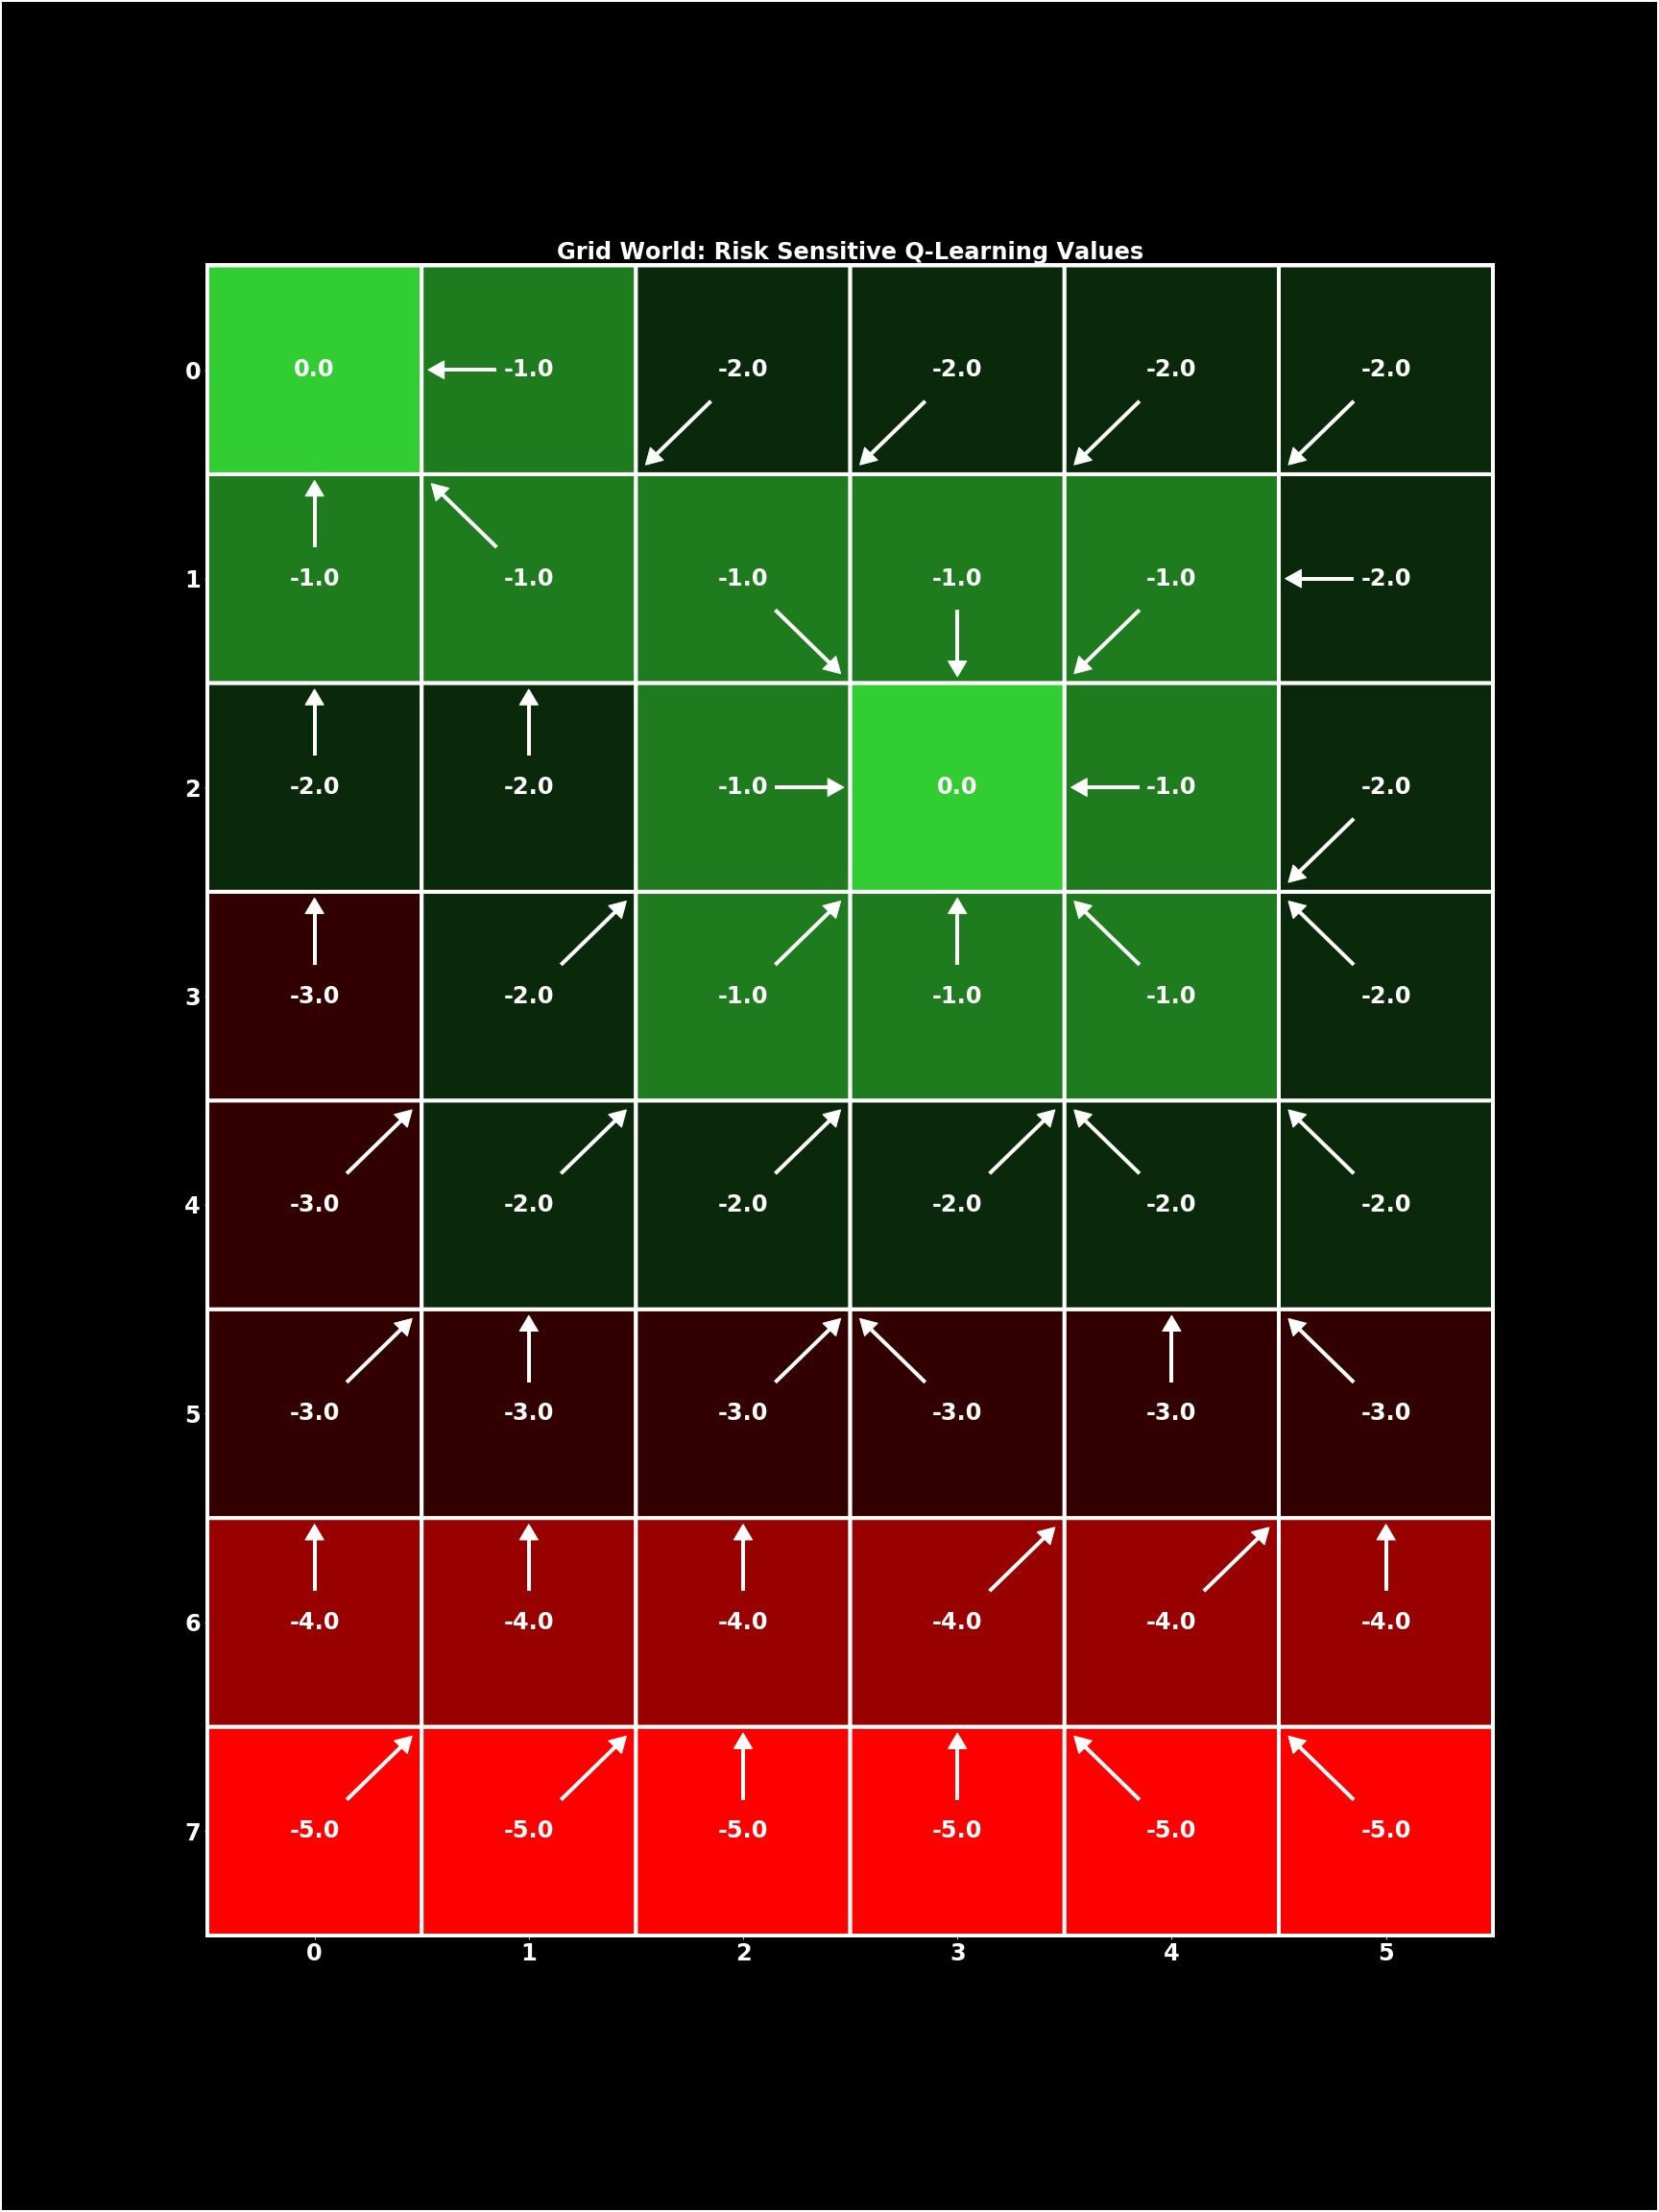
\includegraphics[width=0.5\linewidth]{../figs/Grid_World_Risk_Sensitive_QLearning_Values}\label{fig:sim2}}
    \caption{Risk Sensitive Q-learning results.}
    \label{fig:sim}
\end{figure}


\section{New York Taxi Dataset}
\subsection{Data Description}
The New York Taxi Dataset covers taxi operations from $2010$--$2013$, in total there are nearly $700$ million recorded trips. The data is stored in separate CSV files for each month. We will analyze a subset of the drivers and over only a few months. Each row in a file contains the information for a trip record. The key information that is contained is the hack license (driver ID), pickup date-time, dropoff date-time, trip time in seconds, trip distance in miles, GPS coordinates at the starting location, GPS coordinates at the ending location, total fare including tip, and the total cost of tolls.
\subsection{MDP Formulation for Taxi Drivers}
We model a taxi driver as acting according to a finite MDP where an episode corresponds to a single days work. The complete formulation is given in Section \ref{mdp}. They salient features of the formulation are:
\begin{itemize}
\item Each state is a tuple containing the node the driver is in--we discretized location into a grid using district boundaries for New York City--an indicator of whether the taxi currently is full (just picked up passengers) or empty (just dropped off passengers), and the cumulative reward interval the driver is in--we discretized the reward intervals assuming that how a driver behaves may be a function of the earnings at a point in the workday.
\item Actions are moving between nodes in the location grid we created.
\item The reward functions use values derived from the data, such as earning rate, the expected time searching for a passenger, and the fare between grid nodes. The transition probabilities use empirical transition probabilities as well as expected earning rates. 
\end{itemize}
\subsection{Data Preprocessing}
The data required a significant amount of preprocessing to clean the data and obtain the needed quantities for the MDP formulation. This dataset has been used a fair amount for research and there are some well documented errors. In fact, it was estimated by the folks who obtained the data that nearly $10\%$ of trips contained erroneous information. Below are some of the things we did to clean the data:
\begin{itemize}
\item The trip time reported is often inaccurate. To compensate for this we calculate the trip time using the difference between the reported pickup and dropoff time.
\item We drop the following trip instances: trips that occur in which the GPS coordinates are not in New York, trip times that are extremely short to the point of being infeasible, and trips with extremely low (less than \$.30 a minute) or extremely high (greater than \$20 an hour) earning rates.
\end{itemize}
These are only a subset of the issues with the data that we cleaned but these are the most significant and well documented from previous work with the data. 

There are also a couple of important things we do to create the MDP which we make note of. Drivers work abnormal hours, i.e. the typical driver begins work in the evening and works until the early morning hours. In light of this we shift all transaction times back by 12 hours so that we can observe the full workday within a single date. We estimate the time spent searching for a new trip as the time from dropoff to pickup, but if this time exceeds 20 we assume the driver was taking a break.
\section{Future Work}
As the final deadline approaches we will work on towards the following experiments and goals. First and foremost, utilizing the underlying MDP framework that we have designed for taxi drivers we will investigate the divergence between the empirical policy of drivers found in the data and the optimal policy found with a standard q-learning formulation. This will be allow us to determine whether drivers have learned to maximize their expected earnings. We will then explore the risk-sensitive q-learning formulation, and with the value functions we examine, attempt to find parameters which produce a policy that gives low KL divergence with the empirical policy. If we can do this successfully, it will allow us to characterize how drivers weigh decisions and their risk preferences. Time permitting, we will then explore the risk-sensitive inverse reinforcement learning problem in Grid-World and then in the taxi dataset. 

\bibliographystyle{plainnat}
\bibliography{bibtex}
\section{Appendix}\label{appendix}



\subsection{Risk-Sensitive Decision Making Example}\label{example}
A prevalent example to demonstrate how risk factors into human-decision making including warping of the probability of events as well as losses being weighed more significantly than gains is as follows. When asked to choose between being given \$90 or having a 10\% chance of winning \$100 and a 90\% chance of winning \$0 most people will choose to take the guaranteed \$90. When this question is framed as a loss however, i.e. to choose between losing \$90 or having a 10\% chance of losing \$0 and a 90\% chance of losing \$100, most will choose to risk an increased loss for a chance at no loss. A rational, risk-neutral decision maker would be indifferent to the options in both framings of the question since the expected value of each option is the same.


\subsection{Risk-Sensitive Q-Learning Description}\label{alg_desc}
Q-learning is an off-policy method, meaning the policy being learned is not the policy that is being sampled from when choosing actions to interact with the environment. The policy that is being followed must be proper, meaning that all states are visited infinitely often. Two such proper policies are the $\epsilon$-greedy policy and the Boltzmann policy. Each of these methods trades off exploration and exploitation. Given the greedy action $a^* = \arg \max_a Q(s, a)$ the $\epsilon$-greedy policy is given by
\begin{equation} \pi(a|s) =
\begin{cases}
\ 1 - \epsilon + \frac{\epsilon}{|A|} & a = a^* \\
\frac{\epsilon}{|A|} & a \neq a^*
\end{cases}
\end{equation}
where $\epsilon \in [0, 1]$ controls the greediness. The Boltzmann policy is given by
\begin{equation} \pi(a|s) =
\frac{e^{\tau Q(s, a)}}{\sum_a e^{\tau Q(s, a)}} 
\end{equation}
where $\tau$ is a temperature parameter $\in [0, \infty)$ that controls the greediness. It is common to use a decay rate on the parameters controlling the greediness to make the algorithm more greedy as the environment is further explored. To guarantee convergence of the algorithm the Robbins and Monro conditions \cite{robbins1951stochastic} on the learning rate must hold:
\begin{equation}
\sum_{t=0}^\infty \alpha_t(s, a) = \infty \hspace{5mm} \text{and} \hspace{5mm} \sum_{t=0}^\infty \alpha_t^2(s, a) < \infty, \ \forall \ s, a.
\end{equation}
One such method of choosing the iterates that is common is to let the learning rate be ${\alpha_t(s, a) = 1/N_t(s, a)}$ where $N_t(s, a)$ is the number of times action $a$ has been taken from state $s$. The Q-learning update applying the value function to the temporal difference is given as follows:
\begin{equation}
Q_{t+1}(s_t, a_t) = Q_t(s_t, a_t) + \alpha_t(s_t, a_t)\left[u(r_t + \gamma \max_a Q_t(s_{t+1}, a_t) - Q_t(s_t, a_t))\right].
\end{equation}
See Section \ref{value} for value functions we consider as the nonlinear transformation $u$.



\subsection{Value Functions}\label{value}
We explore several functions that capture risk-sensitive decision making including a prospect theory value function \cite{tversky1992advances} and a logarithm-based value function \cite{mazumdar:2017aa}. The prospect value function is given by:
\begin{equation}u(y) = 
\begin{cases}
c_+ (y)^{\rho^+} & y > 0 \\
-c_- (-y)^{\rho^+} & y \leq 0 \\
\end{cases}
\end{equation}
and the logarithm based value function is given by:
\begin{equation}u(y) = 
\begin{cases}
c_+ \log(1 + \rho^+y)& y > 0 \\
-c_- \log(1 - \rho^+y) & y \leq 0 \\
\end{cases}
\end{equation}
where we are setting the reference point to be 0. The parameters $(c_+, c_-, \rho+, \rho_-)$ control the degree of risk-sensitivity and loss aversion. Typically human decision makers have $0 < \rho_+, \rho_- < 1$. This leads to leads to risk-averse preferences in gains and risk-seeking preferences in losses. In terms of the shape of the function these preferences correspond to concavity in gains and convexity in losses.



\subsection{Further Simulation Results}\label{sim}
Further simulation results are given in Fig.~\ref{fig:sim_more}. In particular we show the reward at each episode which we see see quickly goes towards being optimal, the value of $\epsilon$ from using the $\epsilon$-greedy with decay policy, and learning rate using decay for a state.
\begin{figure}[H]
    \centering
    \subfloat[][Episode Returns.]{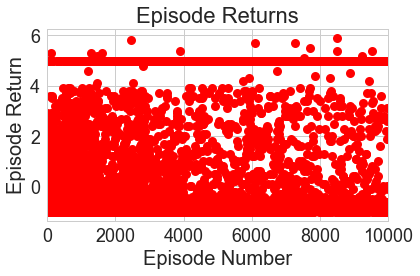
\includegraphics[width=0.33\linewidth]{../figs/Episode_Returns}\label{fig:sim3}}\hfill
    \subfloat[][Epsilon choices.]{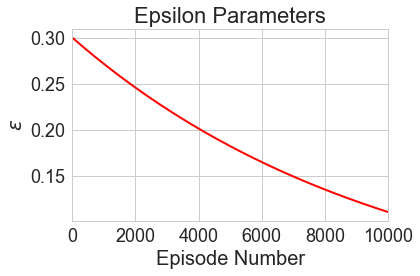
\includegraphics[width=0.33\linewidth]{../figs/Epsilon_Parameters}\label{fig:sim4}}
    \subfloat[][Learning rate choices.]{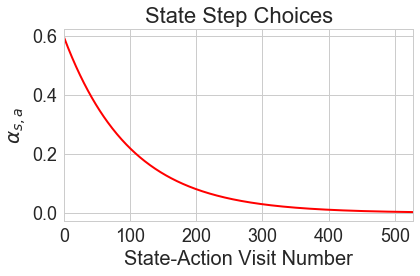
\includegraphics[width=0.33\linewidth]{../figs/State_Step_Choices}\label{fig:sim5}}
    \caption{Detailed Simulation Results.}
    \label{fig:sim_more}
\end{figure}

\subsection{Taxi MDP Model Description}\label{mdp}
\subsubsection{State Space}
The state space is
\[\mc{X}=\{\mc{N}\cup\{x_f\}\times\mc{S}\times \mc{R}\}\backslash \mc{X}_{na}\]
where
\begin{itemize}
\item $x_f$ is the terminal state representing the taxi being done for the period,

\item $\mc{N}$ be the index set for the zones or nodes in the city with $N$ nodes,

\item $\mc{S}=\{${\e, \f}$\}$ is an indicator of if the taxi is \e=empty or \f=full, and

\item $\mc{R}$ is the discretized cumulative fare value space which has the
structure \[\mc{R}=\{\mc{R}_1\}\cup\cdots\cup\{\mc{R}_m\}\cup\{\mc{R}_f\}\]
where $\mc{R}_i=[a_i,b_i]$ with $a_1< b_1\leq a_2<b_2 \cdots \leq a_m<
b_m=\bar{r}$ and $\mc{R}_f=[\bar{r}, \infty)$ where $\bar{r}$ is some reference point for period earnings (e.g., if the period of investigation is a day, then this is the daily earnings reference point).

\item $\mc{X}_{na}$ are the states not allowed and is defined by
\[\mc{X}_{na}=\{(x_f,\f,r), r\in \mc{R}\}\cup\{(x_f,\e,r), r\notin\mc{R}_f\}\]
\end{itemize}
   
A state $(i,s,r)\in \mc{N}\times\mc{S}\times \mc{R}$ indicates the taxi
is in node $i$ (or terminal state $x_f$ if $i=x_f$), has a empty/full state of $s$ and has current cumulative
fare value $r$. The terminal state is reached when the fare value portion of the
state is greater than or equal to $\bar{r}$. 

The dimension of the state space is thus, 
\[(\dim(\mc{N})+\dim(\{x_f\}))\times\dim(\mc{S})\times\dim(\mc{R})-|\mc{X}_{na}|.\]


\subsubsection{Action Space}
Let $\mc{U}=\mc{U}_a\cup\{\emptyset\}$ where
$\mc{U}_a=\{u_{i\mapsto j}, (i,j)\in \mc{N}\times \mc{N}\}$ be the action space where $u_{i\mapsto j}$ indicates the choice of going from node $i$ to node $j$ and where $\emptyset$ is the null action. The admissible actions are state dependent. In particular, if the state is $x=(i,\e,r)$ for any $i\in
\mc{N}$ and any cumulative fare value $r\in\mc{R}$, then $\mc{U}(i,\e,r)=\{u_{i\mapsto j}, (i,j)\in \mc{N}\times \mc{N}\}$ and, on the other hand, if $x=(i,\f,r)$ for any $i\in \mc{N}$ and any cumulative fare value $r\in\mc{R}$, then
$\mc{U}(i,\f,r)=\{\emptyset\}$ indicating that the taxi is currently full and is taking a ride from node $i$ to node $k$ with probability $\Pdest(i,k)$ (i.e.~the probability that a fare picked up in node $i$ will want to go to node $k$).

\subsubsection{Transition Kernel}
Let $\mc{P}: \mc{X}\times \mc{U}\times\mc{X}\rar [0,1]$ be the transition kernel such that $\mc{P}(x_{t},u_t, x_{t+1})$ is the probability that state $x_t$ will transition to state $x_{t+1}$ given action $u_t$. Let's consider the different cases. 
\begin{itemize}
\item First let's look at the $\e$ to $\e$ transitions for all other state action pairs:
\[\mc{P}( (i,\e,r),u,(j,\e,r'))=\left\{\begin{array}{ll} 1, & \ \text{if}\ r,r'\in \mc{R}_f\ \text{\&}\ \{i\in \mc{N},j=x_f\}\vee\{i=x_f,j=x_f\}\\
0, & \ \text{otherwise}\end{array}\right.\]

\item Now let's look at the $\f$ to $\f$ transitions for all other state action pairs:

\[\mc{P}( (i,\f,r),u,(j,\f,r'))=0\]
\item Next we will look at the $\f$ to $\e$ transitions for all other state action pairs:
\[\mc{P}((i,\f,r),u,(j,\e,r'))=\left\{\begin{array}{ll}
\Pdest(i,j)P(E[F(i,j)]+r\geq a_l)\ & \ \text{if}\ r'\in \mc{R}_l, r'\geq r\ \text{\&}\ i,j\in \mc{N}\\ 0, & \ \text{otherwise} \end{array}\right.\]
where $a_l$ is the lower bound on the interval
$\mc{R}_l=[a_l,b_l)$
\item Finally we look at the $\e$ to $\f$ transitions (these are all ones where the choices of action dictates the transition probability)

\[\mc{P}( (i,\e,r),u,(j,\f,r'))=\left\{\begin{array}{ll} 1, & \ \text{if}\ u=u_{i\mapsto j}\ \text{\&}\ r=r', r\notin \mc{R}_f\\
0, & \ \text{otherwise}\end{array}\right.\]
\end{itemize}

\subsubsection{Reward Function}
The reward function is a map $R:\mc{X}\times \mc{U}\times \mc{X}\times \rar \mb{R}$ with $R(x_{t},u_t,x_{t+1})$ a random variable such that
\begin{itemize}
\item The reward for $\f$ to $\e$ is 

\[R( (i,\f,r), u, (j,\e,r'))=\left\{\begin{array}{ll}F(i,j), & \ \text{if}\ i,j\in \mc{N}, u=\emptyset, r'\geq r\\ 0, & \ \text{otherwise}\end{array}\right.\]
where $F(i,j)$ is a random variable representing the fare from $i$ to $j$. 


\item The reward for $\e$ to $\f$ is 
\[R((i,\f,r), u, (j,\e,r'))=\left\{\begin{array}{ll}-t_{\text{\sn{seek}}}(i,j)/E(i,j)^{-1}, & \ \text{if}\ i,j\in \mc{N}, u=u_{i\mapsto j}, r=r'\notin \mc{R}_f\\
0, & \ \text{otherwise}\end{array}\right.\]

where $t_{\text{\sn{seek}}}(i,j)$ is a random variable for the time to travel and find a fare when you go from node $i$ to $j$ under the control action $u_{i\mapsto j}$ and where $E(i,j)$ is a random variable for the earning rate for trips from $i$ to $j$. In practice, we infer the mean values of these quantities from the data.
\end{itemize}

\subsubsection{Initial State}
The intial state for the taxi will be $x_0=(i,\e,r_0)$ where $i$ is the node or
zone which the taxi most frequently starts in and $r_0\in \mc{R}_0=[0,b_0)$. It always starts in the empty state.
\end{document}














